% !TEX encoding = UTF-8 Unicode
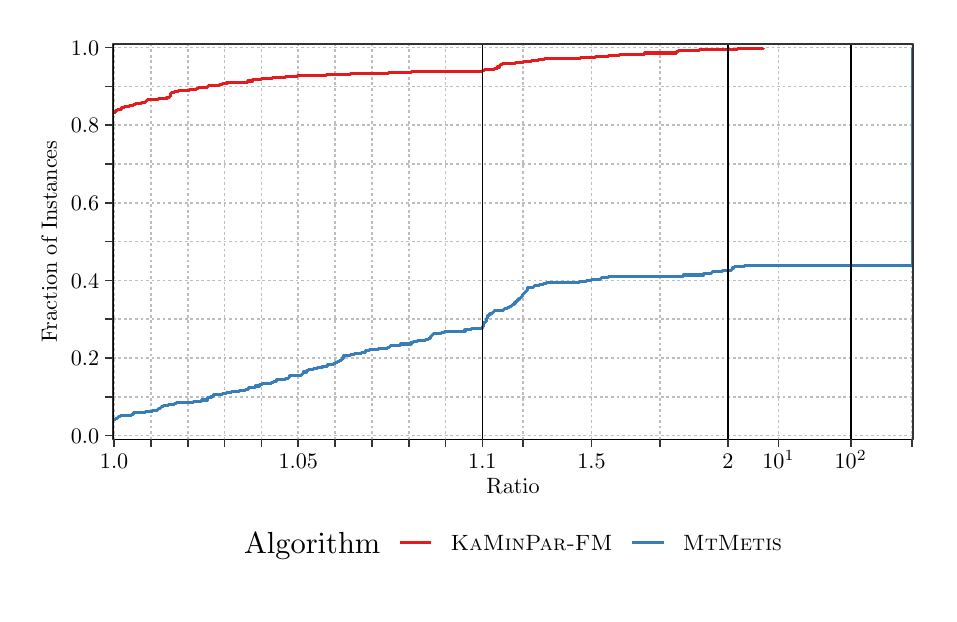
\begin{tikzpicture}[x=1pt,y=1pt]
\definecolor{fillColor}{RGB}{255,255,255}
\begin{scope}
\definecolor{drawColor}{RGB}{255,255,255}
\definecolor{fillColor}{RGB}{255,255,255}

\path[draw=drawColor,line width= 0.6pt,line join=round,line cap=round,fill=fillColor] (  0.00,150.88) rectangle (325.21,355.01);
\end{scope}
\begin{scope}
\definecolor{fillColor}{RGB}{255,255,255}

\path[fill=fillColor] ( 30.48,206.51) rectangle (319.71,349.51);
\definecolor{drawColor}{RGB}{190,190,190}

\path[draw=drawColor,line width= 0.6pt,dash pattern=on 1pt off 1pt ,line join=round] ( 30.48,207.91) --
	(319.71,207.91);

\path[draw=drawColor,line width= 0.6pt,dash pattern=on 1pt off 1pt ,line join=round] ( 30.48,221.93) --
	(319.71,221.93);

\path[draw=drawColor,line width= 0.6pt,dash pattern=on 1pt off 1pt ,line join=round] ( 30.48,235.95) --
	(319.71,235.95);

\path[draw=drawColor,line width= 0.6pt,dash pattern=on 1pt off 1pt ,line join=round] ( 30.48,249.97) --
	(319.71,249.97);

\path[draw=drawColor,line width= 0.6pt,dash pattern=on 1pt off 1pt ,line join=round] ( 30.48,263.99) --
	(319.71,263.99);

\path[draw=drawColor,line width= 0.6pt,dash pattern=on 1pt off 1pt ,line join=round] ( 30.48,278.01) --
	(319.71,278.01);

\path[draw=drawColor,line width= 0.6pt,dash pattern=on 1pt off 1pt ,line join=round] ( 30.48,292.03) --
	(319.71,292.03);

\path[draw=drawColor,line width= 0.6pt,dash pattern=on 1pt off 1pt ,line join=round] ( 30.48,306.05) --
	(319.71,306.05);

\path[draw=drawColor,line width= 0.6pt,dash pattern=on 1pt off 1pt ,line join=round] ( 30.48,320.07) --
	(319.71,320.07);

\path[draw=drawColor,line width= 0.6pt,dash pattern=on 1pt off 1pt ,line join=round] ( 30.48,334.09) --
	(319.71,334.09);

\path[draw=drawColor,line width= 0.6pt,dash pattern=on 1pt off 1pt ,line join=round] ( 30.48,348.11) --
	(319.71,348.11);

\path[draw=drawColor,line width= 0.6pt,dash pattern=on 1pt off 1pt ,line join=round] ( 30.93,206.51) --
	( 30.93,349.51);

\path[draw=drawColor,line width= 0.6pt,dash pattern=on 1pt off 1pt ,line join=round] ( 44.24,206.51) --
	( 44.24,349.51);

\path[draw=drawColor,line width= 0.6pt,dash pattern=on 1pt off 1pt ,line join=round] ( 57.54,206.51) --
	( 57.54,349.51);

\path[draw=drawColor,line width= 0.6pt,dash pattern=on 1pt off 1pt ,line join=round] ( 70.85,206.51) --
	( 70.85,349.51);

\path[draw=drawColor,line width= 0.6pt,dash pattern=on 1pt off 1pt ,line join=round] ( 84.16,206.51) --
	( 84.16,349.51);

\path[draw=drawColor,line width= 0.6pt,dash pattern=on 1pt off 1pt ,line join=round] ( 97.47,206.51) --
	( 97.47,349.51);

\path[draw=drawColor,line width= 0.6pt,dash pattern=on 1pt off 1pt ,line join=round] (110.78,206.51) --
	(110.78,349.51);

\path[draw=drawColor,line width= 0.6pt,dash pattern=on 1pt off 1pt ,line join=round] (124.09,206.51) --
	(124.09,349.51);

\path[draw=drawColor,line width= 0.6pt,dash pattern=on 1pt off 1pt ,line join=round] (137.39,206.51) --
	(137.39,349.51);

\path[draw=drawColor,line width= 0.6pt,dash pattern=on 1pt off 1pt ,line join=round] (150.70,206.51) --
	(150.70,349.51);

\path[draw=drawColor,line width= 0.6pt,dash pattern=on 1pt off 1pt ,line join=round] (164.01,206.51) --
	(164.01,349.51);

\path[draw=drawColor,line width= 0.6pt,dash pattern=on 1pt off 1pt ,line join=round] (178.80,206.51) --
	(178.80,349.51);

\path[draw=drawColor,line width= 0.6pt,dash pattern=on 1pt off 1pt ,line join=round] (203.44,206.51) --
	(203.44,349.51);

\path[draw=drawColor,line width= 0.6pt,dash pattern=on 1pt off 1pt ,line join=round] (228.09,206.51) --
	(228.09,349.51);

\path[draw=drawColor,line width= 0.6pt,dash pattern=on 1pt off 1pt ,line join=round] (252.73,206.51) --
	(252.73,349.51);

\path[draw=drawColor,line width= 0.6pt,dash pattern=on 1pt off 1pt ,line join=round] (270.98,206.51) --
	(270.98,349.51);

\path[draw=drawColor,line width= 0.6pt,dash pattern=on 1pt off 1pt ,line join=round] (297.09,206.51) --
	(297.09,349.51);

\path[draw=drawColor,line width= 0.6pt,dash pattern=on 1pt off 1pt ,line join=round] (319.27,206.51) --
	(319.27,349.51);
\definecolor{drawColor}{RGB}{228,26,28}

\path[draw=drawColor,line width= 1.1pt,line join=round] ( 30.93,324.74) --
	( 31.33,324.74) --
	( 31.33,325.13) --
	( 31.39,325.13) --
	( 31.39,325.52) --
	( 32.33,325.52) --
	( 32.33,325.91) --
	( 33.61,325.91) --
	( 33.61,326.30) --
	( 34.76,326.30) --
	( 34.76,326.69) --
	( 36.57,326.69) --
	( 36.57,327.08) --
	( 38.11,327.08) --
	( 38.11,327.47) --
	( 38.56,327.47) --
	( 38.56,327.86) --
	( 40.86,327.86) --
	( 40.86,328.25) --
	( 42.26,328.25) --
	( 42.26,328.64) --
	( 42.64,328.64) --
	( 42.64,329.03) --
	( 43.13,329.03) --
	( 43.13,329.42) --
	( 46.81,329.42) --
	( 46.81,329.81) --
	( 50.05,329.81) --
	( 50.05,330.19) --
	( 51.08,330.19) --
	( 51.08,330.58) --
	( 51.35,330.58) --
	( 51.35,330.97) --
	( 51.35,330.97) --
	( 51.35,331.36) --
	( 51.80,331.36) --
	( 51.80,331.75) --
	( 52.80,331.75) --
	( 52.80,332.14) --
	( 54.21,332.14) --
	( 54.21,332.53) --
	( 58.01,332.53) --
	( 58.01,332.92) --
	( 60.66,332.92) --
	( 60.66,333.31) --
	( 61.48,333.31) --
	( 61.48,333.70) --
	( 64.83,333.70) --
	( 64.83,334.09) --
	( 65.17,334.09) --
	( 65.17,334.48) --
	( 69.12,334.48) --
	( 69.12,334.87) --
	( 70.12,334.87) --
	( 70.12,335.26) --
	( 71.73,335.26) --
	( 71.73,335.65) --
	( 79.15,335.65) --
	( 79.15,336.04) --
	( 81.09,336.04) --
	( 81.09,336.43) --
	( 84.08,336.43) --
	( 84.08,336.82) --
	( 88.17,336.82) --
	( 88.17,337.20) --
	( 92.80,337.20) --
	( 92.80,337.59) --
	( 97.14,337.59) --
	( 97.14,337.98) --
	(107.74,337.98) --
	(107.74,338.37) --
	(116.26,338.37) --
	(116.26,338.76) --
	(129.91,338.76) --
	(129.91,339.15) --
	(138.47,339.15) --
	(138.47,339.54) --
	(164.05,339.54) --
	(164.05,339.93) --
	(164.86,339.93) --
	(164.86,340.32) --
	(168.46,340.32) --
	(168.46,340.71) --
	(169.36,340.71) --
	(169.36,341.10) --
	(170.30,341.10) --
	(170.30,341.49) --
	(170.63,341.49) --
	(170.63,341.88) --
	(171.26,341.88) --
	(171.26,342.27) --
	(175.84,342.27) --
	(175.84,342.66) --
	(178.87,342.66) --
	(178.87,343.05) --
	(181.79,343.05) --
	(181.79,343.44) --
	(184.39,343.44) --
	(184.39,343.83) --
	(186.59,343.83) --
	(186.59,344.21) --
	(199.46,344.21) --
	(199.46,344.60) --
	(204.73,344.60) --
	(204.73,344.99) --
	(209.44,344.99) --
	(209.44,345.38) --
	(213.72,345.38) --
	(213.72,345.77) --
	(222.72,345.77) --
	(222.72,346.16) --
	(234.13,346.16) --
	(234.13,346.55) --
	(234.80,346.55) --
	(234.80,346.94) --
	(242.38,346.94) --
	(242.38,347.33) --
	(256.34,347.33) --
	(256.34,347.72) --
	(265.51,347.72) --
	(265.51,348.11);
\definecolor{drawColor}{RGB}{55,126,184}

\path[draw=drawColor,line width= 1.1pt,line join=round] ( 30.93,213.75) --
	( 31.42,213.75) --
	( 31.42,214.14) --
	( 32.22,214.14) --
	( 32.22,214.53) --
	( 32.40,214.53) --
	( 32.40,214.92) --
	( 33.41,214.92) --
	( 33.41,215.31) --
	( 37.14,215.31) --
	( 37.14,215.70) --
	( 38.10,215.70) --
	( 38.10,216.09) --
	( 42.26,216.09) --
	( 42.26,216.48) --
	( 44.80,216.48) --
	( 44.80,216.87) --
	( 46.56,216.87) --
	( 46.56,217.26) --
	( 47.07,217.26) --
	( 47.07,217.65) --
	( 47.69,217.65) --
	( 47.69,218.04) --
	( 48.02,218.04) --
	( 48.02,218.42) --
	( 48.81,218.42) --
	( 48.81,218.81) --
	( 50.68,218.81) --
	( 50.68,219.20) --
	( 52.60,219.20) --
	( 52.60,219.59) --
	( 53.34,219.59) --
	( 53.34,219.98) --
	( 59.53,219.98) --
	( 59.53,220.37) --
	( 62.54,220.37) --
	( 62.54,220.76) --
	( 64.59,220.76) --
	( 64.59,221.15) --
	( 64.79,221.15) --
	( 64.79,221.54) --
	( 65.95,221.54) --
	( 65.95,221.93) --
	( 66.73,221.93) --
	( 66.73,222.32) --
	( 66.94,222.32) --
	( 66.94,222.71) --
	( 69.95,222.71) --
	( 69.95,223.10) --
	( 71.52,223.10) --
	( 71.52,223.49) --
	( 73.41,223.49) --
	( 73.41,223.88) --
	( 76.22,223.88) --
	( 76.22,224.27) --
	( 78.47,224.27) --
	( 78.47,224.66) --
	( 79.52,224.66) --
	( 79.52,225.05) --
	( 79.57,225.05) --
	( 79.57,225.43) --
	( 81.89,225.43) --
	( 81.89,225.82) --
	( 83.57,225.82) --
	( 83.57,226.21) --
	( 84.70,226.21) --
	( 84.70,226.60) --
	( 87.87,226.60) --
	( 87.87,226.99) --
	( 88.62,226.99) --
	( 88.62,227.38) --
	( 89.73,227.38) --
	( 89.73,227.77) --
	( 89.74,227.77) --
	( 89.74,228.16) --
	( 93.03,228.16) --
	( 93.03,228.55) --
	( 93.94,228.55) --
	( 93.94,228.94) --
	( 94.14,228.94) --
	( 94.14,229.33) --
	( 94.44,229.33) --
	( 94.44,229.72) --
	( 98.54,229.72) --
	( 98.54,230.11) --
	( 99.04,230.11) --
	( 99.04,230.50) --
	( 99.27,230.50) --
	( 99.27,230.89) --
	(100.61,230.89) --
	(100.61,231.28) --
	(101.21,231.28) --
	(101.21,231.67) --
	(102.95,231.67) --
	(102.95,232.06) --
	(104.47,232.06) --
	(104.47,232.44) --
	(106.06,232.44) --
	(106.06,232.83) --
	(108.07,232.83) --
	(108.07,233.22) --
	(108.11,233.22) --
	(108.11,233.61) --
	(110.23,233.61) --
	(110.23,234.00) --
	(111.08,234.00) --
	(111.08,234.39) --
	(111.75,234.39) --
	(111.75,234.78) --
	(112.41,234.78) --
	(112.41,235.17) --
	(113.20,235.17) --
	(113.20,235.56) --
	(113.37,235.56) --
	(113.37,235.95) --
	(113.71,235.95) --
	(113.71,236.34) --
	(113.87,236.34) --
	(113.87,236.73) --
	(116.27,236.73) --
	(116.27,237.12) --
	(117.69,237.12) --
	(117.69,237.51) --
	(120.32,237.51) --
	(120.32,237.90) --
	(121.85,237.90) --
	(121.85,238.29) --
	(121.92,238.29) --
	(121.92,238.68) --
	(123.12,238.68) --
	(123.12,239.07) --
	(126.43,239.07) --
	(126.43,239.45) --
	(129.76,239.45) --
	(129.76,239.84) --
	(130.35,239.84) --
	(130.35,240.23) --
	(130.90,240.23) --
	(130.90,240.62) --
	(134.48,240.62) --
	(134.48,241.01) --
	(138.21,241.01) --
	(138.21,241.40) --
	(139.03,241.40) --
	(139.03,241.79) --
	(140.58,241.79) --
	(140.58,242.18) --
	(143.32,242.18) --
	(143.32,242.57) --
	(144.53,242.57) --
	(144.53,242.96) --
	(145.29,242.96) --
	(145.29,243.35) --
	(145.40,243.35) --
	(145.40,243.74) --
	(145.66,243.74) --
	(145.66,244.13) --
	(145.85,244.13) --
	(145.85,244.52) --
	(146.20,244.52) --
	(146.20,244.91) --
	(149.17,244.91) --
	(149.17,245.30) --
	(150.39,245.30) --
	(150.39,245.69) --
	(157.72,245.69) --
	(157.72,246.08) --
	(160.11,246.08) --
	(160.11,246.46) --
	(164.13,246.46) --
	(164.13,246.85) --
	(164.21,246.85) --
	(164.21,247.24) --
	(164.25,247.24) --
	(164.25,247.63) --
	(164.34,247.63) --
	(164.34,248.02) --
	(164.39,248.02) --
	(164.39,248.41) --
	(164.44,248.41) --
	(164.44,248.80) --
	(165.25,248.80) --
	(165.25,249.19) --
	(165.60,249.19) --
	(165.60,249.58) --
	(165.63,249.58) --
	(165.63,249.97) --
	(165.64,249.97) --
	(165.64,250.36) --
	(165.77,250.36) --
	(165.77,250.75) --
	(165.78,250.75) --
	(165.78,251.14) --
	(166.55,251.14) --
	(166.55,251.53) --
	(166.76,251.53) --
	(166.76,251.92) --
	(167.72,251.92) --
	(167.72,252.31) --
	(168.17,252.31) --
	(168.17,252.70) --
	(168.55,252.70) --
	(168.55,253.09) --
	(171.63,253.09) --
	(171.63,253.47) --
	(172.06,253.47) --
	(172.06,253.86) --
	(173.00,253.86) --
	(173.00,254.25) --
	(173.89,254.25) --
	(173.89,254.64) --
	(174.65,254.64) --
	(174.65,255.03) --
	(174.92,255.03) --
	(174.92,255.42) --
	(175.44,255.42) --
	(175.44,255.81) --
	(175.90,255.81) --
	(175.90,256.20) --
	(176.70,256.20) --
	(176.70,256.59) --
	(176.76,256.59) --
	(176.76,256.98) --
	(177.23,256.98) --
	(177.23,257.37) --
	(177.62,257.37) --
	(177.62,257.76) --
	(178.29,257.76) --
	(178.29,258.15) --
	(178.52,258.15) --
	(178.52,258.54) --
	(178.65,258.54) --
	(178.65,258.93) --
	(178.75,258.93) --
	(178.75,259.32) --
	(179.16,259.32) --
	(179.16,259.71) --
	(179.56,259.71) --
	(179.56,260.10) --
	(179.83,260.10) --
	(179.83,260.48) --
	(180.37,260.48) --
	(180.37,260.87) --
	(180.39,260.87) --
	(180.39,261.26) --
	(182.54,261.26) --
	(182.54,261.65) --
	(182.79,261.65) --
	(182.79,262.04) --
	(184.81,262.04) --
	(184.81,262.43) --
	(186.06,262.43) --
	(186.06,262.82) --
	(187.02,262.82) --
	(187.02,263.21) --
	(199.18,263.21) --
	(199.18,263.60) --
	(201.77,263.60) --
	(201.77,263.99) --
	(203.52,263.99) --
	(203.52,264.38) --
	(206.55,264.38) --
	(206.55,264.77) --
	(207.12,264.77) --
	(207.12,265.16) --
	(209.56,265.16) --
	(209.56,265.55) --
	(236.64,265.55) --
	(236.64,265.94) --
	(244.00,265.94) --
	(244.00,266.33) --
	(246.94,266.33) --
	(246.94,266.72) --
	(247.07,266.72) --
	(247.07,267.11) --
	(250.75,267.11) --
	(250.75,267.49) --
	(254.08,267.49) --
	(254.08,267.88) --
	(254.49,267.88) --
	(254.49,268.27) --
	(254.57,268.27) --
	(254.57,268.66) --
	(255.20,268.66) --
	(255.20,269.05) --
	(258.65,269.05) --
	(258.65,269.44) --
	(319.27,269.44) --
	(319.27,342.27) --
	(319.27,342.27) --
	(319.27,348.11);
\definecolor{drawColor}{RGB}{0,0,0}

\path[draw=drawColor,line width= 0.6pt,line join=round] (164.01,206.51) -- (164.01,349.51);

\path[draw=drawColor,line width= 0.6pt,line join=round] (252.73,206.51) -- (252.73,349.51);

\path[draw=drawColor,line width= 0.6pt,line join=round] (297.09,206.51) -- (297.09,349.51);
\definecolor{drawColor}{gray}{0.20}

\path[draw=drawColor,line width= 0.6pt,line join=round,line cap=round] ( 30.48,206.51) rectangle (319.71,349.51);
\end{scope}
\begin{scope}
\definecolor{drawColor}{RGB}{0,0,0}

\path[draw=drawColor,line width= 0.2pt,line join=round] ( 30.48,206.51) --
	( 30.48,349.51);
\end{scope}
\begin{scope}
\definecolor{drawColor}{RGB}{0,0,0}

\node[text=drawColor,anchor=base east,inner sep=0pt, outer sep=0pt, scale=  0.80] at ( 25.53,205.16) {0.0};

\node[text=drawColor,anchor=base east,inner sep=0pt, outer sep=0pt, scale=  0.80] at ( 25.53,233.19) {0.2};

\node[text=drawColor,anchor=base east,inner sep=0pt, outer sep=0pt, scale=  0.80] at ( 25.53,261.23) {0.4};

\node[text=drawColor,anchor=base east,inner sep=0pt, outer sep=0pt, scale=  0.80] at ( 25.53,289.27) {0.6};

\node[text=drawColor,anchor=base east,inner sep=0pt, outer sep=0pt, scale=  0.80] at ( 25.53,317.31) {0.8};

\node[text=drawColor,anchor=base east,inner sep=0pt, outer sep=0pt, scale=  0.80] at ( 25.53,345.35) {1.0};
\end{scope}
\begin{scope}
\definecolor{drawColor}{gray}{0.20}

\path[draw=drawColor,line width= 0.6pt,line join=round] ( 27.73,207.91) --
	( 30.48,207.91);

\path[draw=drawColor,line width= 0.6pt,line join=round] ( 27.73,221.93) --
	( 30.48,221.93);

\path[draw=drawColor,line width= 0.6pt,line join=round] ( 27.73,235.95) --
	( 30.48,235.95);

\path[draw=drawColor,line width= 0.6pt,line join=round] ( 27.73,249.97) --
	( 30.48,249.97);

\path[draw=drawColor,line width= 0.6pt,line join=round] ( 27.73,263.99) --
	( 30.48,263.99);

\path[draw=drawColor,line width= 0.6pt,line join=round] ( 27.73,278.01) --
	( 30.48,278.01);

\path[draw=drawColor,line width= 0.6pt,line join=round] ( 27.73,292.03) --
	( 30.48,292.03);

\path[draw=drawColor,line width= 0.6pt,line join=round] ( 27.73,306.05) --
	( 30.48,306.05);

\path[draw=drawColor,line width= 0.6pt,line join=round] ( 27.73,320.07) --
	( 30.48,320.07);

\path[draw=drawColor,line width= 0.6pt,line join=round] ( 27.73,334.09) --
	( 30.48,334.09);

\path[draw=drawColor,line width= 0.6pt,line join=round] ( 27.73,348.11) --
	( 30.48,348.11);
\end{scope}
\begin{scope}
\definecolor{drawColor}{RGB}{0,0,0}

\path[draw=drawColor,line width= 0.2pt,line join=round] ( 30.48,206.51) --
	(319.71,206.51);
\end{scope}
\begin{scope}
\definecolor{drawColor}{gray}{0.20}

\path[draw=drawColor,line width= 0.6pt,line join=round] ( 30.93,203.76) --
	( 30.93,206.51);

\path[draw=drawColor,line width= 0.6pt,line join=round] ( 44.24,203.76) --
	( 44.24,206.51);

\path[draw=drawColor,line width= 0.6pt,line join=round] ( 57.54,203.76) --
	( 57.54,206.51);

\path[draw=drawColor,line width= 0.6pt,line join=round] ( 70.85,203.76) --
	( 70.85,206.51);

\path[draw=drawColor,line width= 0.6pt,line join=round] ( 84.16,203.76) --
	( 84.16,206.51);

\path[draw=drawColor,line width= 0.6pt,line join=round] ( 97.47,203.76) --
	( 97.47,206.51);

\path[draw=drawColor,line width= 0.6pt,line join=round] (110.78,203.76) --
	(110.78,206.51);

\path[draw=drawColor,line width= 0.6pt,line join=round] (124.09,203.76) --
	(124.09,206.51);

\path[draw=drawColor,line width= 0.6pt,line join=round] (137.39,203.76) --
	(137.39,206.51);

\path[draw=drawColor,line width= 0.6pt,line join=round] (150.70,203.76) --
	(150.70,206.51);

\path[draw=drawColor,line width= 0.6pt,line join=round] (164.01,203.76) --
	(164.01,206.51);

\path[draw=drawColor,line width= 0.6pt,line join=round] (178.80,203.76) --
	(178.80,206.51);

\path[draw=drawColor,line width= 0.6pt,line join=round] (203.44,203.76) --
	(203.44,206.51);

\path[draw=drawColor,line width= 0.6pt,line join=round] (228.09,203.76) --
	(228.09,206.51);

\path[draw=drawColor,line width= 0.6pt,line join=round] (252.73,203.76) --
	(252.73,206.51);

\path[draw=drawColor,line width= 0.6pt,line join=round] (270.98,203.76) --
	(270.98,206.51);

\path[draw=drawColor,line width= 0.6pt,line join=round] (297.09,203.76) --
	(297.09,206.51);

\path[draw=drawColor,line width= 0.6pt,line join=round] (319.27,203.76) --
	(319.27,206.51);
\end{scope}
\begin{scope}
\definecolor{drawColor}{RGB}{0,0,0}

\node[text=drawColor,anchor=base,inner sep=0pt, outer sep=0pt, scale=  0.80] at ( 30.93,196.05) {$1.0$};

\node[text=drawColor,anchor=base,inner sep=0pt, outer sep=0pt, scale=  0.80] at ( 44.24,196.05) {$$};

\node[text=drawColor,anchor=base,inner sep=0pt, outer sep=0pt, scale=  0.80] at ( 57.54,196.05) {$$};

\node[text=drawColor,anchor=base,inner sep=0pt, outer sep=0pt, scale=  0.80] at ( 70.85,196.05) {$$};

\node[text=drawColor,anchor=base,inner sep=0pt, outer sep=0pt, scale=  0.80] at ( 84.16,196.05) {$$};

\node[text=drawColor,anchor=base,inner sep=0pt, outer sep=0pt, scale=  0.80] at ( 97.47,196.05) {$1.05$};

\node[text=drawColor,anchor=base,inner sep=0pt, outer sep=0pt, scale=  0.80] at (110.78,196.05) {$$};

\node[text=drawColor,anchor=base,inner sep=0pt, outer sep=0pt, scale=  0.80] at (124.09,196.05) {$$};

\node[text=drawColor,anchor=base,inner sep=0pt, outer sep=0pt, scale=  0.80] at (137.39,196.05) {$$};

\node[text=drawColor,anchor=base,inner sep=0pt, outer sep=0pt, scale=  0.80] at (150.70,196.05) {$$};

\node[text=drawColor,anchor=base,inner sep=0pt, outer sep=0pt, scale=  0.80] at (164.01,196.05) {$1.1$};

\node[text=drawColor,anchor=base,inner sep=0pt, outer sep=0pt, scale=  0.80] at (178.80,196.05) {$$};

\node[text=drawColor,anchor=base,inner sep=0pt, outer sep=0pt, scale=  0.80] at (203.44,196.05) {$1.5$};

\node[text=drawColor,anchor=base,inner sep=0pt, outer sep=0pt, scale=  0.80] at (228.09,196.05) {$$};

\node[text=drawColor,anchor=base,inner sep=0pt, outer sep=0pt, scale=  0.80] at (252.73,196.05) {$2$};

\node[text=drawColor,anchor=base,inner sep=0pt, outer sep=0pt, scale=  0.80] at (270.98,196.05) {$10^1$};

\node[text=drawColor,anchor=base,inner sep=0pt, outer sep=0pt, scale=  0.80] at (297.09,196.05) {$10^2$};

\node[text=drawColor,anchor=base,inner sep=0pt, outer sep=0pt, scale=  0.80] at (319.27,196.05) {\symbInfeasible};
\end{scope}
\begin{scope}
\definecolor{drawColor}{RGB}{0,0,0}

\node[text=drawColor,anchor=base,inner sep=0pt, outer sep=0pt, scale=  0.80] at (175.10,187.01) {Ratio};
\end{scope}
\begin{scope}
\definecolor{drawColor}{RGB}{0,0,0}

\node[text=drawColor,rotate= 90.00,anchor=base,inner sep=0pt, outer sep=0pt, scale=  0.80] at ( 10.23,278.01) {Fraction of Instances};
\end{scope}
\begin{scope}
\definecolor{drawColor}{RGB}{0,0,0}

\node[text=drawColor,anchor=base,inner sep=0pt, outer sep=0pt, scale=  1.10] at (102.51,165.32) {Algorithm};
\end{scope}
\begin{scope}
\definecolor{fillColor}{RGB}{255,255,255}

\path[fill=fillColor] (132.61,161.88) rectangle (147.07,176.33);
\end{scope}
\begin{scope}
\definecolor{drawColor}{RGB}{228,26,28}

\path[draw=drawColor,line width= 1.1pt,line join=round] (134.06,169.11) -- (145.62,169.11);
\end{scope}
\begin{scope}
\definecolor{fillColor}{RGB}{255,255,255}

\path[fill=fillColor] (216.53,161.88) rectangle (230.99,176.33);
\end{scope}
\begin{scope}
\definecolor{drawColor}{RGB}{55,126,184}

\path[draw=drawColor,line width= 1.1pt,line join=round] (217.98,169.11) -- (229.54,169.11);
\end{scope}
\begin{scope}
\definecolor{drawColor}{RGB}{0,0,0}

\node[text=drawColor,anchor=base west,inner sep=0pt, outer sep=0pt, scale=  0.80] at (152.57,166.35) {\textsc{KaMinPar-FM}};
\end{scope}
\begin{scope}
\definecolor{drawColor}{RGB}{0,0,0}

\node[text=drawColor,anchor=base west,inner sep=0pt, outer sep=0pt, scale=  0.80] at (236.49,166.35) {\textsc{MtMetis}};
\end{scope}
\end{tikzpicture}
